\documentclass[11pt,a4paper]{article}

\usepackage[margin=2.4cm]{geometry}
\usepackage{graphicx}
\usepackage{booktabs}
\usepackage{caption}
\usepackage{subcaption}
\usepackage{float}
\usepackage{xcolor}
\usepackage{listings}
\usepackage{enumitem}
\usepackage[hidelinks]{hyperref}
\usepackage{titlesec}

\definecolor{accent}{HTML}{2166AC}
\definecolor{codebg}{HTML}{F5F5F3}
\definecolor{inksoft}{HTML}{5C5A54}

\titleformat{\section}{\large\bfseries\color{accent}}{\thesection}{0.6em}{}
\titleformat{\subsection}{\normalsize\bfseries}{\thesubsection}{0.6em}{}
\titlespacing{\section}{0pt}{1.4em}{0.5em}

\captionsetup{font=small,labelfont={bf,color=accent}}

\lstset{
  backgroundcolor=\color{codebg},
  basicstyle=\ttfamily\footnotesize,
  breaklines=true,
  frame=none,
  xleftmargin=0.6em,
  framexleftmargin=0.6em,
  aboveskip=0.8em,
  belowskip=0.8em,
}

\setlist[itemize]{itemsep=1pt,topsep=3pt,leftmargin=1.2em}

\title{\vspace{-1.4cm}\textbf{Sydney Housing Price Prediction and\\Decision Support System}}
\author{Shalok Sharma \\ \small SIT307 Machine Learning, 8.1 Distinction Task}
\date{\small September 2026}

\begin{document}
\maketitle

\section{Part 1: Problem Definition and Data Collection}

A real estate agency needs a tool that estimates sale price from listed
attributes and is honest about the confidence each deserves. Three
suburbs span different markets: Mosman, premium and harbourside;
Parramatta, a middle ring apartment centre; and Liverpool, an affordable
outer corridor, distinct in Table~\ref{tab:collect}.

Listings were collected by hand from the sold sections of
realestate.com.au and domain.com.au. No crawler was run, since both
sites prohibit automated scraping and the task asks for manual
construction. Every row stores its listing URL and collection date, so
any figure here is traceable, and a blank means the listing published
nothing, never an estimate.

Cleaning mattered: fifteen properties appeared on both sites under
different URLs and would each have carried double weight across
validation folds.

\begin{table}[H]
\centering
\small
\caption{Collection and cleaning, and the resulting suburb markets}
\label{tab:collect}
\begin{tabular}{lr@{\hskip 2.2em}lrr}
\toprule
\textbf{Stage} & \textbf{Rows} & \textbf{Suburb} & \textbf{Properties} & \textbf{Median price} \\
\midrule
Collected from both sites   & 250 & Mosman     & 78 & \$1{,}251{,}250 \\
Duplicated across sites     & $-15$ & Parramatta & 70 & \$600{,}000 \\
Non standard dwelling type  & $-4$  & Liverpool  & 80 & \$538{,}500 \\
Stored dataset              & 231 & & & \\
Removed in cleaning         & $-3$  & & & \\
\textbf{Used for modelling} & \textbf{228} & & & \\
\bottomrule
\end{tabular}
\end{table}

\subsection{Quality, bias and limitations}

\begin{itemize}
  \item \textbf{Apartments dominate}, 195 of 228 rows against 21 houses,
  with no Parramatta houses, leaving house pricing poorly learnt.
  \item \textbf{No description text}, forfeiting the optional text data
  extension.
  \item \textbf{Area is sparsely reported} and, as Part 2 shows, meant
  two different things.
  \item \textbf{One market period}, all sales within 206 days.
\end{itemize}

\section{Part 2: Data Understanding and Feature Engineering}

Prices are heavily right skewed, at 4.6, driven by Mosman sales reaching
\$23{,}000{,}000. Logs reduce this to 0.6 (Figure~\ref{fig:dist}), the
most consequential decision in Part 3.

\begin{figure}[H]
\centering
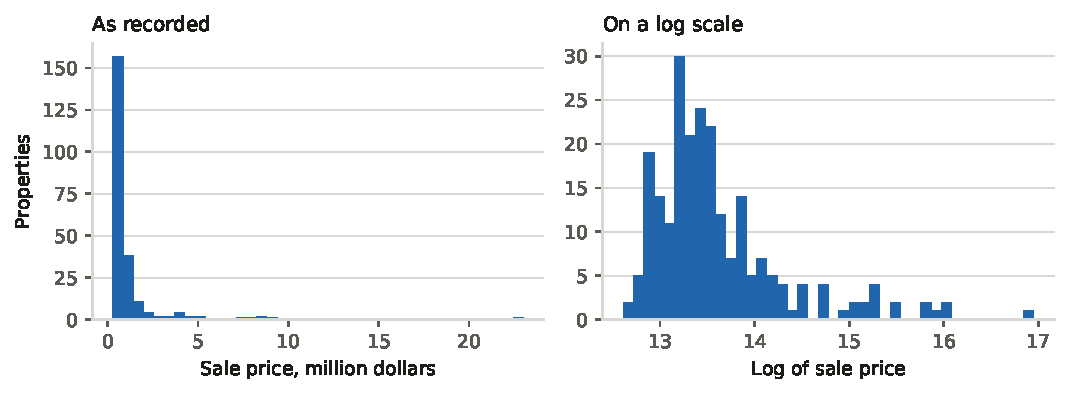
\includegraphics[width=\textwidth]{figures/fig_price_distribution.pdf}
\caption{Sale price as recorded and on a log scale. The long right tail
is what makes the raw target difficult to model.}
\label{fig:dist}
\end{figure}

\begin{figure}[H]
\centering
\begin{subfigure}[t]{0.46\textwidth}
  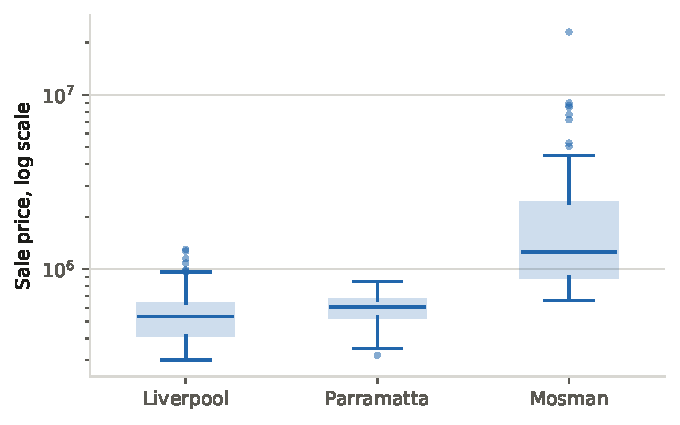
\includegraphics[width=\textwidth]{figures/fig_price_by_suburb.pdf}
  \caption{Price by suburb}
  \label{fig:suburb}
\end{subfigure}
\hfill
\begin{subfigure}[t]{0.50\textwidth}
  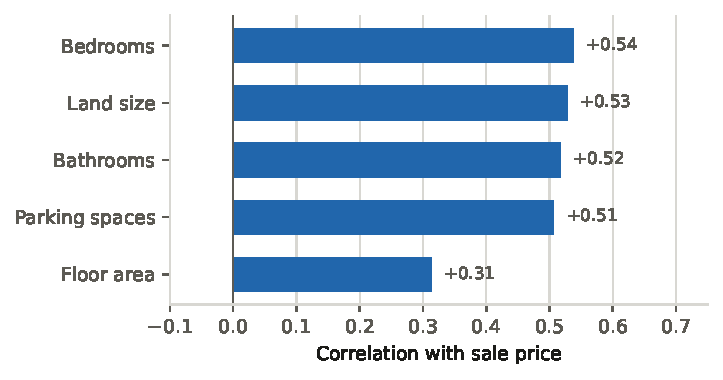
\includegraphics[width=\textwidth]{figures/fig_correlations.pdf}
  \caption{Correlation of each attribute with price}
  \label{fig:corr}
\end{subfigure}
\caption{Three separated markets, and attributes that each explain far
less than the suburb does.}
\end{figure}

\subsection{Two findings that changed the feature set}

Both sites report an area figure, but it is land for a house and floor
area for an apartment, and both arrived in one column. Left together the
model would read the gap between roughly 600 and 100 square metres as a
land effect when it is really house against flat, so it was split by
property type.

Sale date looked useful, correlating at $-0.40$, apparently a sharp
market fall. Within each suburb that collapses towards zero: Mosman
spans the full window while the others cover only its recent third, so
an early date stood in for Mosman, the expensive suburb. The trend
describes collection, not the market, and was excluded.

\subsection{Expected drivers and engineered features}

The three attributes expected to matter most were suburb, whose medians
differ fourfold; property type; and bedrooms. Figure~\ref{fig:corr}
supports this, every attribute correlating far more weakly than the
suburb gaps imply. Distance to the city was excluded as it duplicates
the suburb label exactly. Engineered features are modest: the area
split, and bathrooms per bedroom.

\section{Part 3: Model Development and Evaluation}

Three approaches were compared: ridge linear regression as an
interpretable baseline, a random forest for interactions between suburb,
type and size, and gradient boosting as usually the strongest on
structured data. Both trees were expected to beat the baseline clearly.

The target was tested first. Predicting log price improves every model
and rescues gradient boosting from an $R^2$ of 0.047 to 0.544, because
on raw dollars the squared error is dominated by a few multi million
dollar sales. All results use five fold cross validation on that target,
scored back in dollars.

\begin{table}[H]
\centering
\small
\caption{Five fold cross validation. The two $R^2$ columns describe the
same predictions, measured in log space and in dollars.}
\label{tab:models}
\begin{tabular}{lrrrrr}
\toprule
\textbf{Model} & \textbf{Log $R^2$} & \textbf{Train $R^2$} & \textbf{Gap} & \textbf{Dollar $R^2$} & \textbf{Median error} \\
\midrule
Linear Regression & 0.869 & 0.906 & 0.038 & 0.402 & 14.5\% \\
Random Forest     & 0.872 & 0.961 & 0.089 & \textbf{0.537} & \textbf{11.4\%} \\
Gradient Boosting & \textbf{0.876} & 0.962 & 0.086 & 0.544 & 11.7\% \\
\bottomrule
\end{tabular}
\end{table}

The expectation was only partly correct. On the log scale all three are
almost indistinguishable, linear regression falling within 0.01 of both
trees while showing the smallest train and test gap. With seven features
and no text, little non linear structure remains, because logs already
convert multiplicative price behaviour into something additive. The
trees separate only on the dollar metrics, which weight expensive errors
heavily. Random forest is recommended: its 11.4\% median error is lowest
and is the metric the tool reports. Quoting only the log $R^2$ of 0.87
would overstate it; 0.54 is what matters to somebody handed a price.

\section{Part 4: Investigating Prediction Failures}

\begin{table}[H]
\centering
\small
\caption{The five largest errors, from cross validated predictions}
\label{tab:errors}
\begin{tabular}{llrrrr}
\toprule
\textbf{Property} & \textbf{Type} & \textbf{Beds} & \textbf{Sold} & \textbf{Predicted} & \textbf{Error} \\
\midrule
17 Morella Road    & House     & 4 & \$23{,}000{,}000 & \$5{,}200{,}000 & 77\% \\
34 Rickard Avenue  & House     & 7 & \$9{,}000{,}000  & \$4{,}700{,}000 & 48\% \\
96 Glover Street   & House     & 4 & \$3{,}390{,}000  & \$7{,}300{,}000 & 116\% \\
5 Botanic Road     & House     & 4 & \$8{,}700{,}000  & \$5{,}300{,}000 & 39\% \\
G05 Myahgah Road   & Apartment & 2 & \$4{,}500{,}000  & \$1{,}700{,}000 & 62\% \\
\bottomrule
\end{tabular}
\end{table}

All five are in Mosman and the errors run both ways: three trophy houses
under predicted, 96 Glover Street over predicted by more than double,
and the fifth sold for four times the Mosman apartment median, almost
certainly a penthouse but recorded as a two bedroom flat.

The common thread is not that these are expensive but that in Mosman the
recorded attributes stop discriminating. Only 13 Mosman houses span
\$3{,}390{,}000 to \$23{,}000{,}000 and six publish no land size, so the
model separates them on bedroom counts that barely differ. Position,
outlook and build quality set these prices, and none are in the data.

Figure~\ref{fig:err} quantifies it: 21.2\% median error in Mosman
against 8.2\% and 9.7\% elsewhere, not because Mosman is costly but
because its stock is heterogeneous with few comparable sales. The most
valuable missing information is recent comparable street sales, what a
valuer consults first.

\begin{figure}[H]
\centering
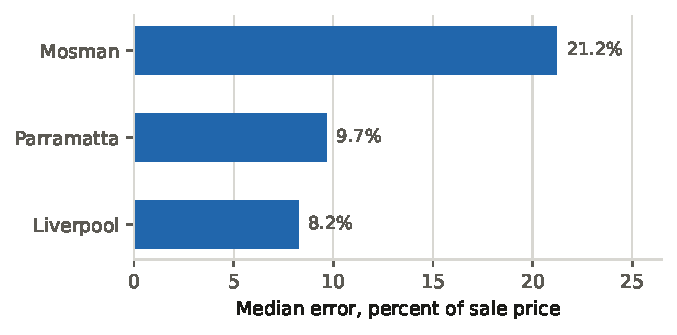
\includegraphics[width=0.62\textwidth]{figures/fig_error_by_suburb.pdf}
\caption{Median percentage error by suburb, from cross validated
predictions. Mosman is roughly two and a half times harder.}
\label{fig:err}
\end{figure}

\section{Part 5: Final Deployment and Reflection}

\subsection{How the application was built}

The tool is a Flask application, keeping prediction logic in one small
Python file while the page stays plain HTML and CSS, so it runs with no
build step. On start it loads the saved random forest and a schema of
the feature list, per suburb error rates and thin combinations.

Three decisions shape it. Inputs are validated on the server, where
untrusted data enters. The result is a range, set by that suburb's cross
validated median error. And it refuses to bluff: asked for a Parramatta
house it says so (Figure~\ref{fig:warn}).

\begin{figure}[H]
\centering
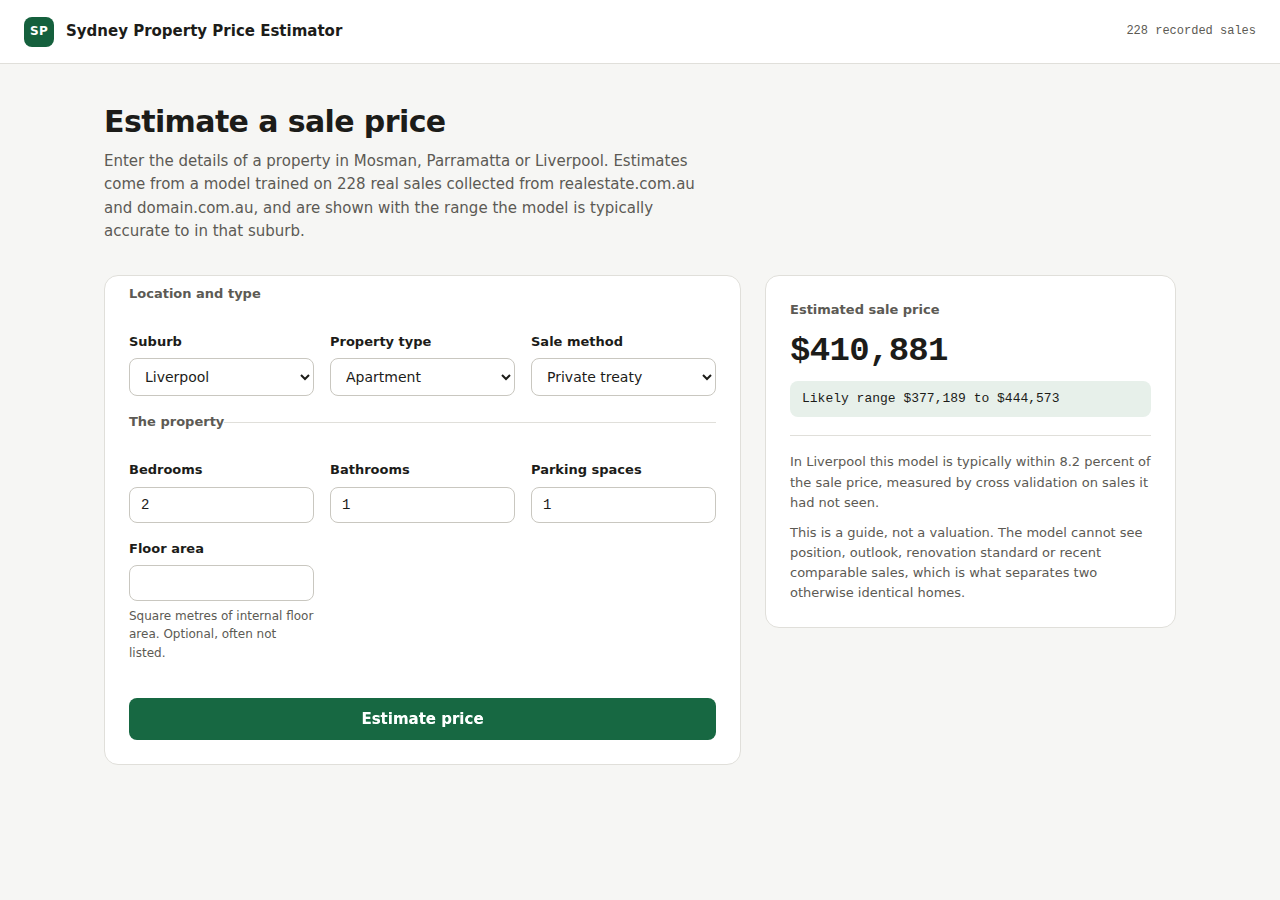
\includegraphics[width=0.86\textwidth]{figures/app_result.png}
\caption{The application estimating a Liverpool apartment. The range
comes from the 8.2\% median error measured for that suburb.}
\label{fig:app}
\end{figure}

\begin{figure}[H]
\centering
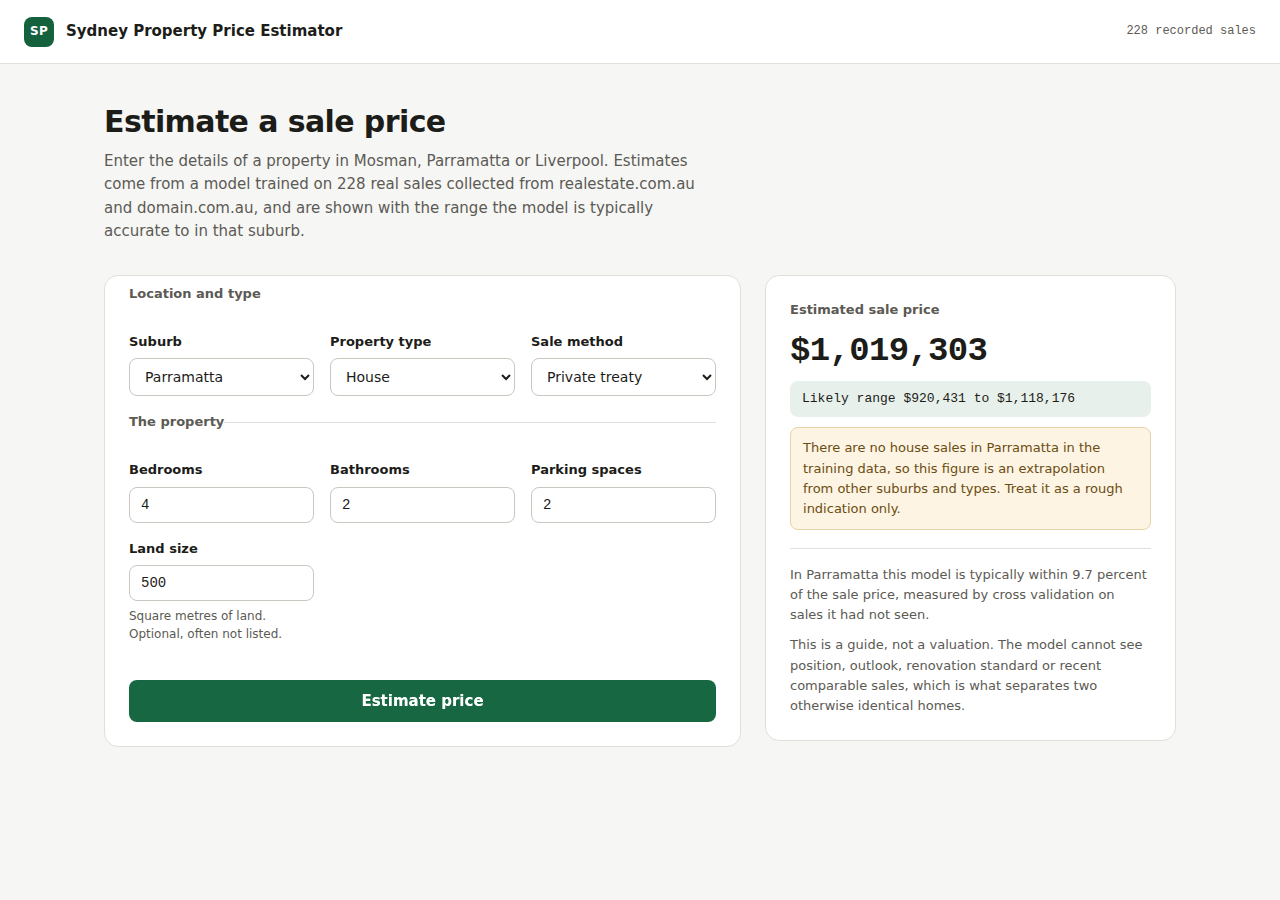
\includegraphics[width=0.86\textwidth]{figures/app_low_confidence_warning.png}
\caption{Asked for a Parramatta house, a combination absent from the
training data, the tool warns instead of answering confidently.}
\label{fig:warn}
\end{figure}

\subsection{Building and running it}

\begin{lstlisting}[language=bash]
pip install -r requirements.txt

# Rebuild the dataset, features and notebook
python3 scripts/prepare_features.py
jupyter nbconvert --to notebook --execute --inplace \
        notebooks/sydney_housing_price_prediction.ipynb

# Run the web application, then open http://127.0.0.1:5000
python3 app/flask_app.py
\end{lstlisting}

Select a suburb and type, enter the attributes and press Estimate price.
Choosing a house switches the area field from floor area to land size.

\subsection{Reflection}

The lessons came from the data, not the algorithms. The findings above
surfaced only because results were checked rather than accepted, none
were visible in summary statistics, and each would have quietly damaged
the model. Choosing the log target mattered more than the algorithm.

Accuracy is unevenly distributed, dependable for Liverpool and
Parramatta apartments and unreliable for Mosman houses. Presenting both
with equal confidence would mislead a buyer precisely where the sums are
largest, which is why the tool reports suburb ranges and flags thin
combinations. The dataset is also 85\% strata.

With more time the priorities would be collecting the descriptions and
build years listing pages publish, balancing property types, and adding
comparable street sales.

\section*{Acknowledgement of GenAI use}

Claude, an AI coding assistant, was used for planning and for writing
and reviewing code across the notebook, collection tooling and web
application. Every number, table and figure here comes from executing
that code on the collected data; none were estimated. The analytical
decisions are explained in the text above.

\section*{Code and data}

All code, the dataset, the notebook and the application are at:

\begin{center}
\url{https://github.com/Shalok-sys/Sydney-Housing-Price-Prediction}
\end{center}

\noindent It contains \texttt{data/} (collected listings and cleaned
table), \texttt{notebooks/} (full analysis with visible outputs),
\texttt{scripts/} (collection, validation, feature pipeline),
\texttt{app/} (the Flask application) and \texttt{models/}.

\begin{thebibliography}{9}
\small
\bibitem{sklearn} Pedregosa, F. et al. (2011). Scikit learn: Machine
Learning in Python. \textit{Journal of Machine Learning Research}, 12,
pp. 2825 to 2830.
\bibitem{breiman} Breiman, L. (2001). Random Forests.
\textit{Machine Learning}, 45(1), pp. 5 to 32.
\bibitem{rea} realestate.com.au (2026). Sold property listings, Mosman,
Parramatta and Liverpool NSW. Accessed September 2026.
\bibitem{domain} domain.com.au (2026). Sold property listings, Mosman,
Parramatta and Liverpool NSW. Accessed September 2026.
\end{thebibliography}

\end{document}
